\documentclass[12pt,a4paper,openright,twoside]{book}
\usepackage[utf8]{inputenc}
\usepackage{amsmath}
\usepackage{amssymb}
\usepackage{listings}
\usepackage{algpseudocode}
\usepackage{tabularx}
\usepackage{graphics}
\usepackage{disi-thesis}
\usepackage{code-lstlistings}
\usepackage{notes}
\usepackage{shortcuts}
\usepackage{acronym}
\usepackage[linesnumbered,ruled,vlined]{algorithm2e}


\newcommand{\thesislang}{english} % commentare in caso di tesi in italiano
%\usepackage{thesis-style}
% version
%\newcommand{\versionmajor}{0}
%\newcommand{\versionminor}{1}
%\newcommand{\versionpatch}{2}
%\newcommand{\version}{\versionmajor.\versionminor.\versionpatch}
%\typeout{Document version: \version}

\school{\unibo}
\programme{Corso di Laurea Magistrale in Ingegneria e Scienze Informatiche}
\title{Fair-by-design algoriths for access to education}
\author{Antonio Iannotta}
\date{\today}
\subject{Intelligent Systems Engineering}
\supervisor{Prof. Giovanni Ciatto}
\cosupervisor{Prof. Roberta Calegari}
\morecosupervisor{Prof. Andrea Omicini}
\session{IV}
\academicyear{2022-2023}

% Definition of acronyms
\acrodef{IoT}{Internet of Thing}
\acrodef{vm}[VM]{Virtual Machine}
\acrodef{AI}{Artificial Intelligence}


\mainlinespacing{1.241} % line spacing in mainmatter, comment to default

\begin{document}
	
\frontmatter

% ! TeX root = thesis-main.tex
\title{Title}
\author{Candidate Name Here}
\date{\today}

\newgeometry{margin=0.8in}
\begin{titlepage}
	\begin{center}
		% \vspace*{0.2cm}
		
		\large
		\textbf{ALMA MATER STUDIORUM -- UNIVERSITÀ DI BOLOGNA \\ CAMPUS DI CESENA}
		\\
		\noindent\hrulefill
		\vspace{0.4cm}
		
		\Large
		Scuola di Ingegneria e Architettura \\
		Corso di Laurea Magistrale in Ingegneria e Scienze Informatiche
		
		\Huge
		\vspace{4cm}
		\textbf{
			Fair-by-design algorithm for access to education
		}
		
		\large
		\vspace{1cm}
		Tesi di laurea in 
		\\
		\textsc{Intelligent System Engineering}
		
		\vspace{5.5cm}
		\begin{minipage}[t]{0.64\textwidth}
			\begin{flushleft}
				\textit{Relatore} 
				\\ 
				\textbf{Prof.} \textbf{Giovanni Ciatto}
				\\
				\vspace{0.4cm}
				\textit{Correlatore} 
				\\
				\textbf{Prof.} \textbf{Roberta Calegari}
				\textbf{Prof.} \textbf{Andre Omicini}
			\end{flushleft}
		\end{minipage}
		\begin{minipage}[t]{0.34\textwidth}
			\begin{flushright}
				\textit{Candidato} 
				\\ 
				\textbf{Antonio Iannotta}
			\end{flushright}
		\end{minipage}\\
		
		\vfill
		\noindent\hrulefill
		\vspace{0.3cm}
		\Large
		
		IV Sessione di Laurea
		\\
		Anno Accademico 2022-2023
	\end{center}
\end{titlepage}
\restoregeometry


\begin{abstract}

    This work presents an in-depth approach to address fairness and bias mitigation in the design and development of data-driven methods. The primary contribution of this study is the proposal and implementation of an innovative \emph{Fair-by-Design} workflow that incorporates various strategies for bias mitigation within data, algorithms, and decision-making processes.

    The work focuses on the educational data of the Canary Islands, leveraging a dataset encompassing detailed information about student performance and educational outcomes.

    The primary objective is to ensure equitable and unbiased application of data-driven algorithms within the educational context. 

    The methodology involves the systematic evaluation of multiple bias mitigation strategies. The critical aspect of this research centers on the comparison of these strategies based on their impact on the predictive accuracy of the algorithms. 

    This approach provides practical insights into the trade-offs between fairness and accuracy, showing how several approaches can lead to different accuracy scores on the same dataset and with the same models. 

    The work findings offer valuable insights into the trade-offs between fairness and accuracy when developing data-driven methods for educational data. 

    This thesis contributes to the ongoing discourse on fairness in machine learning and data-driven decision-making. The results provide guidance for stakeholders in the education sector, aiding them in making informed decisions about algorithm deployment to promote fairness and minimize bias within educational systems. 

\end{abstract}
    


%\begin{acknowledgements} % this is optional
%Never too far down, to come back
%\end{acknowledgements}

%----------------------------------------------------------------------------------------
\tableofcontents   
%\listoffigures     % (optional) comment if empty
%\lstlistoflistings % (optional) comment if empty
%----------------------------------------------------------------------------------------

\mainmatter

%----------------------------------------------------------------------------------------
\chapter{Introduction}
\label{chap:introduction}
%----------------------------------------------------------------------------------------

Artificial Intelligence (AI) has experienced an unprecedented surge in prominence and utility in recent years, emerging as a transformative force across diverse domains. From powering autonomous vehicles to aiding healthcare diagnosis and recommendation systems, AI applications have become increasingly woven into the fabric of our daily lives. However, this rapid proliferation has ushered in a pressing concern about the pervasive presence of bias within AI systems.

The concept of bias in AI pertains to the inadvertent or systematic preference shown towards specific groups or characteristics within the data, algorithms, or decision-making processes. This partiality leads to outcomes that are unjust, unfair, and unequal. In this era of AI-driven decision-making, the imperative to address bias is not just a technological challenge but a moral and societal necessity. Additionally, the ethical principle of fairness underscores the collective aspiration to ensure that AI systems yield equitable and just results for all individuals, regardless of their personal attributes.

The repercussions of bias and unfairness in AI systems extend far beyond mere technological concerns. These issues carry profound societal implications, impacting vital areas such as employment, education, and access to critical services. Biased AI systems perpetuate and exacerbate existing inequalities, inadvertently reinforcing harmful stereotypes and undermining the foundational principles of justice and equality. 

In the realm of education, data-driven decision-making has gained significant ground, with educational institutions increasingly relying on AI systems for tasks ranging from student admissions to evaluating learning outcomes and allocating educational resources. The stakes in this domain are notably high. Ensuring that these AI-driven education systems mitigate bias and prioritize fairness is not just a technological endeavor; it is a moral and societal imperative. 

This work introduces a comprehensive Fair-by-Design workflow, meticulously detailed in the \textbf{Contribution} chapter. The crux of this workflow is its unique ability to integrate fairness considerations right from the inception of AI system design. In this thesis, we rigorously explore and implement three distinct and promising approaches to ensure fairness, together with the well-known \emph{fairness through unawareness} approach, with the goal to compare the accuracy derived by the application of each approach with the usual scenario in which fairness assumptions are not made. 

These approaches are seamlessly integrated into the workflow, facilitating a comprehensive and unbiased comparison of their effectiveness in mitigating bias. 

The structure of this thesis unfolds as follows: The \textbf{State of the Art} chapter conducts a thorough review of the existing approaches and methodologies designed to address bias and promote fairness in the development of AI systems. This chapter lays the groundwork upon which our innovative Fair-by-Design workflow is built. The \textbf{Contribution} chapter delves into the intricacies of the workflow, elucidating the seamless integration of various fairness approaches into the design process. The \textbf{Validation} chapter meticulously presents the results derived from the application of these fairness approaches, offering an empirical comparison of their performance and effectiveness. Finally, the \textbf{Conclusion} chapter not only imparts insights gleaned from our research but also outlines prospective directions for further advancements in this critical and ever-evolving field.

%----------------------------------------------------------------------------------------
\chapter{State of the Art} % or Background
\label{chap:background}

This chapter provides a comprehensive overview of the preceding works and the scientific literature that have paved the way for the implementation of fair-by-design methods in our research. The journey begins with a thorough examination of the multifaceted field of \textbf{artificial intelligence} and its wide-ranging applications, including its pivotal roles in critical sectors and socio-technical systems. Within this context, we delve deeply into the intricate issues of \textbf{bias} and \textbf{fairness} in AI systems, acknowledging the essential foundation upon which our work is built. 

Artificial Intelligence (\textbf{AI}) stands at the forefront of technological innovation, significantly reshaping diverse sectors, from healthcare to finance and transportation. To comprehensively grasp the transformative potential of AI, it is essential to explore its applications and the complex ecosystems in which it operates. This chapter endeavors to unravel the intricate web of AI systems and their profound impact on society.

However, the proliferation of AI brings with it the inherent challenge of bias. As AI systems learn from vast datasets, they may inadvertently perpetuate and exacerbate existing prejudices, resulting in \textbf{bias} within the algorithms. Recognizing this challenge as a critical one, our exploration extends into the various dimensions of bias, highlighting its multifaceted nature and the potential consequences it carries. 

Moreover, in our quest for equitable AI, the concept of \textbf{fairness} emerges as a beacon of hope. This chapter dissects the concept of fairness within AI systems, exploring the intricate ethical considerations that underlie the pursuit of equitable outcomes for all individuals. The chapter further investigates technical dimensions of fairness, acknowledging that it is not merely a goal but a fundamental ethical principle that underpins our work. 

Through this comprehensive exploration, we pave the way for the implementation of fair-by-design methods. This chapter is not only a testament to the foundation on which our research stands but also a testament to the complexity of the AI landscape, its potential for societal transformation, and the imperative of mitigating bias and promoting fairness as we forge ahead in the development of AI systems. 


\section{Artificial Intelligence}
This chapter embarks on a deep dive into the dynamic and multifaceted realm of Artificial Intelligence (AI) and Machine Learning (ML), two groundbreaking technologies that are reshaping human interaction with the world. AI, as a vast and encompassing domain, denotes the development of computer systems endowed with the capability to perform tasks traditionally reserved for human intelligence. These tasks span the spectrum from speech recognition to intricate problem-solving and adaptive learning. 

Within the expansive domain of AI, Machine Learning emerges as a prominent subset, taking center stage in this exploration. Machine Learning is a field that focuses on creating algorithms that empower computers to discern intricate patterns within data and make informed predictions. At its core, Machine Learning excels at enhancing performance over time by processing and assimilating data. The essence of Machine Learning lies in its ability to autonomously learn from data, continuously adapting and improving its decision-making capabilities. 

The AI and ML landscape encompasses a diverse array of techniques and methodologies. Notable examples include Natural Language Processing, Computer Vision, Robotics, and Expert Systems, each wielding distinct capabilities and applications. Machine Learning, in particular, is a repository of algorithms crafted to enable machines to self-learn and refine their performance sans explicit programming. These algorithms grant machines the ability to make data-driven decisions, essentially automating the process of pattern recognition and prediction. 

The transformative impact of AI extends far beyond the horizon, with direct implications for critical sectors, including healthcare and autonomous driving, where the consequences are not merely abstract but can be a matter of life and death. However, the profound influence of AI is not confined to these sectors alone. It permeates socio-technical systems, which are emblematic of the intricate interplay between individuals, technology, and social institutions. 

Socio-technical systems are marked by the intricate interplay between individuals, technology, and social institutions. AI and ML have catalyzed substantial transformations within these systems, profoundly altering how individuals interact with technology and reshaping the fabric of society. As AI becomes increasingly embedded in the social fabric, it is imperative to confront the intricate ethical quandaries it raises. 

The integration of AI and ML within these systems has precipitated a cascade of intricate ethical dilemmas. These encompass concerns surrounding data privacy, the pervasive presence of biases inherent in algorithms, and the impending potential for job displacement due to automation. In this context, constructing robust ethical frameworks is not just a matter of academic discourse but an essential imperative. 

These ethical frameworks serve as a safeguard, ensuring that AI systems adhere to the principles of fairness, transparency, and accountability. They stand as the bulwark against potential harm and serve to distribute the benefits of AI equitably across society. As this chapter unfolds, it endeavors to delve deeper into these ethical considerations, offering insights into how technology and ethics converge in the evolving landscape of AI and ML. \cite{GRUETZEMACHER202210288}. \cite{GRUETZEMACHER202210288}.

\newpage
\section{Bias}
Artificial Intelligence (AI) is undeniably a transformative force, poised to reshape multiple dimensions of our existence in profound ways. Its versatile applications extend far and wide, from refining and expediting decision-making processes to seamlessly automating mundane and repetitive tasks. In this ever-evolving landscape, AI systems are becoming increasingly integrated into our daily experiences, orchestrating a paradigm shift in how we interact with the world around us. 

However, amidst the excitement and optimism surrounding AI's potential, a growing concern resonates both within the AI community and society as a whole. This concern revolves around the pervasive issue of biases intricately woven into the very fabric of AI algorithms. 

These biases, often unintentional and subtle, can seep into AI systems through the data they are trained on and the methods employed to develop them. As AI systems learn from historical data, they may inadvertently inherit the prejudices and stereotypes present in those datasets. Consequently, these biases can manifest in various ways, perpetuating and amplifying societal inequalities. For example, in AI applications for hiring or lending, biases can result in unfair discrimination based on factors such as race or gender. In automated content recommendations, biases can reinforce echo chambers, limiting exposure to diverse perspectives and ideas. 

The consequences of these biases are far-reaching and profound. They not only undermine the ethical foundations of AI but can also erode trust in these technologies. As AI systems gain prominence in critical areas like healthcare, criminal justice, and education, the ramifications of bias become increasingly worrisome. 

Addressing bias in AI is a complex and ongoing challenge. It requires a multifaceted approach that encompasses not only improved data collection and curation but also transparency in AI decision-making processes. Researchers and engineers are working tirelessly to develop techniques for bias detection and mitigation. Additionally, there is a growing push for diverse representation in the AI development community to ensure that the creation of AI systems considers a wide array of perspectives. 

In conclusion, while the promise of AI is immense, the journey towards harnessing its potential responsibly and equitably is an imperative one. As we move forward in this AI-driven era, it is essential to remain vigilant in identifying and rectifying biases, ensuring that AI truly serves as a force for positive change in our evolving world. \cite{10.1145/3308560.3317590}

\subsection{Understanding Bias in AI}
Bias in AI is a critical issue, signifying the presence of unjust and skewed representations or treatment of individuals or groups based on attributes such as race, gender, age, socioeconomic status, or other defining characteristics. These biases are deeply embedded in AI systems and can persist throughout their development and training processes. They arise from a variety of sources, including historical data imbalances, deeply ingrained societal prejudices, and imperfections in the algorithms themselves.

\subsection{Sources of Bias}
\subsubsection{Historical data} 
The issue of bias originating from historical data is a critical and intricate challenge that looms large in the landscape of machine learning. When machine learning models are trained on datasets culled from the annals of history, they inevitably inherit the biases and patterns encoded within that data. These historical biases, often a reflection of deeply ingrained societal prejudices and structural inequalities, can persist and intensify when the model is operationalized. \cite{10.1145/3308560.3317590}

Consider a scenario where historical data contains systemic biases against specific demographics, such as gender, race, or other socio-demographic attributes. The machine learning model, in its quest to optimize performance, dutifully replicates and perpetuates these biases in its predictions and decision-making processes. The consequence of this perpetuation is the perpetuation of historical injustices, potentially leading to the endorsement of discriminatory practices and the exacerbation of preexisting societal inequalities, significantly disadvantaging certain groups. 

Effectively addressing bias originating from historical data necessitates a multidimensional approach, coupled with proactive measures. The first step involves diligent data preprocessing techniques aimed at the identification and subsequent mitigation of bias-laden elements within the dataset. These techniques span a spectrum from data re-sampling to re-weighting and data augmentation, designed to restore balance and fairness. 

Simultaneously, interventions in algorithmic fairness are introduced to the machine learning process. These interventions encompass a range of techniques, including re-weighting of training instances, the introduction of fairness constraints, and adversarial debiasing methods, all aimed at guiding the model toward making fair and equitable predictions. 

Moreover, the journey toward equitable AI is an ongoing one, requiring constant vigilance. Continuous monitoring and adjustment of models, often in real-time, become imperative to ensure that fairness is upheld and biased outcomes are identified and rectified. 

Ultimately, the overarching goal is to foster a future where machine learning not only learns from historical data but actively works to transcend the bonds of bias. In this vision, AI systems operate as champions of fairness and social justice, contributing to the construction of a more equitable and just society where decisions and predictions are untainted by historical prejudices. This endeavor is not just a technical challenge but a moral imperative, driving the AI community to build a more equitable future for all.

\subsubsection{Human bias}
Bias introduced by human factors represents a pervasive and intricate challenge within the realm of machine learning. It is essential to understand that human bias, which can emanate from societal, cultural, or personal beliefs and attitudes, has the potential to inadvertently permeate the entire spectrum of the machine learning pipeline. This influence spans from the initial stages of data collection and annotation to the model training and decision-making processes. 

Human bias can manifest in multifarious ways, thereby complicating the quest for fair and unbiased machine learning models. These manifestations may include the biased selection of training data, subjectivity in annotations, or implicit prejudices that insidiously seep into the very fabric of algorithm design and evaluation. When humans are intricately involved in the decision-making processes or contribute to the development of algorithms, their biases, often unperceived, can become unintentionally embedded in the model. This results in a cascade of skewed predictions and the inadvertent reinforcement of preexisting societal inequalities. \cite{https://doi.org/10.1002/widm.1356} 

The recognition and mitigation of human bias represent an imperative for the development of equitable and just machine learning models. This mission encompasses several facets. First and foremost, it demands an elevated level of awareness within the machine learning community and society at large. Recognizing the potential pitfalls of human bias is a crucial step toward addressing them. 

Promoting diversity and inclusion, both in the workforce and in the datasets used for model training, is instrumental in countering human bias. Diverse perspectives and a multiplicity of experiences contribute to a more comprehensive and unbiased understanding of the world. 

Moreover, practical measures are implemented to detect and mitigate bias throughout the machine learning pipeline. This includes strategies ranging from fairness-aware machine learning algorithms to post-processing techniques that rectify biased predictions. 

The journey toward mitigating human bias is continuous and iterative. Machine learning practitioners continually refine their algorithms to minimize the impact of human bias and ensure that their models contribute to a more equitable and unbiased society. The ultimate goal is to harness the transformative potential of machine learning while eliminating the inadvertent perpetuation of human biases, thereby ushering in a more equitable and just era in technological advancement.

\subsubsection{Algorithmic bias}

Algorithmic bias, an intrinsic challenge in the domain of machine learning, underscores the presence of inherent biases that can manifest in the design, development, and deployment of machine learning algorithms. These biases, often unintended, can originate from a myriad of sources, encompassing factors such as biased training data, skewed feature selection, or implicit assumptions woven into the algorithm's development process. 

Algorithmic bias possesses the insidious potential to perpetuate and magnify preexisting societal prejudices and disparities, culminating in outcomes that are patently unfair and discriminatory. Consider the scenario in which a machine learning model is trained on historical data that inherently encapsulates societal biases. The model, in its endeavor to optimize predictive accuracy, inadvertently assimilates and reinforces these biases. The result is an algorithm that produces predictions and decisions that are tinged with bias, potentially aggravating societal inequalities and offering unequal treatment to specific groups. \cite{10.1145/2983270} 

Addressing algorithmic bias is a pivotal imperative when striving to construct equitable and just AI systems. This undertaking encompasses a comprehensive scrutiny of the entire machine learning pipeline, from data collection to model development and deployment. It commences with the meticulous assessment and rectification of bias within training data, aiming to restore balance and fairness. 

Furthermore, the integration of fairness-aware algorithms within the machine learning process is crucial. These algorithms are deliberately designed to recognize and rectify biases, offering a safeguard against discriminatory predictions and decisions. 

Transparency and fairness represent integral aspects of the decision-making process. The incorporation of these elements ensures that algorithms operate equitably, are devoid of bias, and actively promote fairness and equal treatment for all individuals, irrespective of their backgrounds. 

In essence, the mission of addressing algorithmic bias is pivotal for harnessing the true potential of AI systems. It involves forging a future where AI, far from perpetuating biases, serves as a champion of fairness and social justice, contributing to the construction of an equitable and just society in the digital age.


\subsection{Example of Bias in AI}
\subsubsection{Race and Gender Bias in Facial Recognition} \cite{https://doi.org/10.5281/zenodo.4050457}
Race and gender bias in facial recognition technology is a pressing and deeply concerning issue that underscores the ethical complexities tied to the development of AI. Facial recognition systems, often trained on large datasets, inadvertently perpetuate biases present in these datasets, particularly biases related to race and gender. The lack of diversity in training data, which is predominantly skewed towards certain demographics, results in algorithmic bias, where the system may struggle to accurately recognize individuals from underrepresented racial or gender groups. 

Studies have provided compelling evidence that these systems are often more accurate for individuals with lighter skin tones compared to those with darker skin tones, demonstrating a clear racial bias. Similarly, gender recognition algorithms may exhibit inaccuracies, especially for gender-nonconforming individuals, further exacerbating biases. 

The consequences of these biases are wide-ranging and profound. For instance, in law enforcement applications, the use of facial recognition may lead to the disproportionate targeting and misidentification of individuals from minority communities, potentially resulting in wrongful arrests and increased surveillance. In commercial contexts, biased facial recognition can significantly impact hiring processes, access to services, and overall societal fairness, with far-reaching implications for individuals and communities.


\subsubsection{Criminal Justice Bias}
Criminal justice bias is a deeply ingrained issue within the legal system that manifests through unequal treatment of individuals based on their race, socioeconomic status, gender, and other factors. The criminal justice system should ideally operate on principles of fairness, justice, and equality before the law. However, biases at various stages of the criminal justice process, from policing and arrest to trial and sentencing, often lead to discriminatory outcomes. \cite{doi:10.1080/10345329.2019.1658694} 

Racial bias is a significant concern, with people of color, especially Black individuals and communities, experiencing disproportionately higher rates of arrest, harsher sentencing, and a lack of trust in the system. Discriminatory practices such as racial profiling and racial disparities in sentencing contribute to this bias. Socioeconomic bias is another critical factor, where individuals from marginalized and low-income communities may face prejudice in the form of limited access to legal resources and unequal treatment within the legal process. \cite{9660177}  

Gender bias is prevalent, particularly against women and gender-diverse individuals. Women can face stereotypes and discriminatory attitudes that affect their treatment by law enforcement, the courts, and correctional facilities. Additionally, biases against LGBTQ+ individuals can result in unfair treatment and disparities in the criminal justice system. \cite{gebru2020race} 

Addressing criminal justice bias necessitates comprehensive reform. This includes implementing policies to combat racial and socioeconomic disparities, providing anti-bias training to law enforcement, encouraging diversity within the legal profession, and promoting transparency and accountability in the criminal justice process. Legislation, sentencing reform, community engagement, and the support of marginalized communities are also vital steps toward achieving a fair and impartial criminal justice system that upholds the principles of equity and justice for all.


\subsubsection{Recruitment Bias}
Recruitment bias is a critical issue within the hiring process, where unconscious or conscious prejudices and preconceived notions influence decision-making during candidate selection. It manifests in various forms, such as racial, gender, age, socio-economic, educational, or even appearance-based biases, and can significantly impact the composition of the workforce. \cite{mujtaba2019ethical} 

One of the most prevalent forms of recruitment bias is racial or ethnic bias. Hiring decisions can be influenced by stereotypes, leading to the underrepresentation of certain racial or ethnic groups in the workplace. Similarly, gender bias can result in disparities in hiring and promotion opportunities, favoring one gender over another. Age bias often affects older candidates who may be overlooked in favor of younger, perceived to be more 'tech-savvy' individuals. 

Educational and socio-economic biases can also seep into the hiring process, where candidates from prestigious institutions or privileged backgrounds may be given preferential treatment. Appearance-based biases, although highly unfortunate, can influence decisions, impacting individuals based on their physical attributes, such as weight, height, or even hairstyle. 

Addressing recruitment bias requires a multipronged approach. Firstly, raising awareness and providing training on unconscious bias is essential for hiring teams. Implementing structured and standardized interview processes, blind recruitment techniques (removing personally identifiable information), and diverse interview panels can help mitigate biases. Moreover, organizations should focus on promoting diversity and inclusion, fostering a culture that values different perspectives and backgrounds, and monitoring and analyzing recruitment data to identify patterns of bias. Striving for fairness and inclusivity in the hiring process not only leads to a more diverse workforce but also improves organizational innovation, creativity, and overall success.
\newpage
\section{Fairness} 
The pursuit of fairness within AI systems represents a dynamic and indispensable area of focus within the ever-expanding realm of artificial intelligence. At its core, fairness underscores an ethical and moral imperative to ensure that AI technologies and algorithms treat all individuals with equitable respect, devoid of bias or discrimination. As AI increasingly penetrates diverse facets of society, from decision-making processes to job recruitment, lending, and law enforcement, the salience of fairness is unequivocal. 

The pursuit of fairness in AI is an all-encompassing endeavor, entailing an array of considerations that orbit around the ambition to eliminate bias predicated on attributes such as race, gender, age, ethnicity, and socio-economic status. Bias in AI manifests in multifarious ways, originating from the training data's inherent biases or the algorithms themselves. Fair AI systems, therefore, endeavor to minimize these biases, upholding the principles of impartiality and justice in the outcomes they produce. 

In the quest for fairness, various fairness metrics and criteria have emerged, serving as quantifiable benchmarks for assessing the equity of AI systems. These include disparate impact, equal opportunity, and demographic parity. Disparate impact assesses the differential impact an AI system has on distinct demographic groups, while equal opportunity guarantees that the probability of a positive outcome remains consistent across all demographic segments. Demographic parity, on the other hand, centers on the proportional representation of various groups within AI-generated outcomes. 

Addressing fairness within AI systems necessitates the employment of an assortment of techniques. This involves pre-processing data to ameliorate biases, the modification of algorithms to instill them with fairness-awareness, and post-processing methods to ensure that outcomes are equitable. Furthermore, transparency and explainability are pivotal features of AI models, facilitating a deeper understanding of potential biases and nurturing trust in the technology. 

Emphasizing the ethical dimension, the pursuit of fairness in AI systems transcends the confines of technical solutions. It necessitates the active involvement of stakeholders, the incorporation of diverse perspectives, and a steadfast commitment to adhering to guidelines and regulations that prioritize fairness and impartiality. 

In essence, the journey to achieve fairness in AI systems is an ongoing and multifaceted odyssey, demanding relentless research, interdisciplinary collaboration, and unwavering ethical vigilance. The ultimate objective is the creation of AI technologies that steadfastly uphold the principles of fairness, contributing to a more inclusive, just, and equitable society. The continued pursuit of fairness in AI is not just a technical endeavor but a moral imperative, shaping the future of technology and its impact on society.
\subsection{Fairness Techniques in AI}

\subsubsection{Pre-processing}
Pre-processing focuses onThe pre-processing phase, an integral component of AI system development, is dedicated to the meticulous handling of data before it is utilized in the training of an AI model. This stage assumes paramount importance as it lays the foundation for equitable and unbiased AI systems, ensuring that the data used is both balanced and representative of the rich diversity inherent in the population. 

The objective of pre-processing is to rectify any imbalances, biases, or irregularities in the data, aiming to foster an environment where the AI model can operate without predisposition. The use of common pre-processing techniques is pivotal to this endeavor. These techniques encompass oversampling and undersampling, which seek to redress the imbalance in the distribution of data across various classes or groups. 

Additionally, pre-processing includes the meticulous removal of noise from the data. Noise, in this context, refers to extraneous or irrelevant information that could distort the model's learning process. The elimination of such noise serves to enhance the data's signal-to-noise ratio, improving the model's ability to discern meaningful patterns. 

Furthermore, the creation of balanced synthetic datasets is a valuable technique within the pre-processing repertoire. This involves the generation of new data points, often through the extrapolation of existing data, with the goal of augmenting the representation of underrepresented classes or groups. 

In summation, pre-processing is the cornerstone of equitable and unbiased AI system development. It encompasses a suite of techniques designed to foster balanced and representative data, enabling AI models to operate with impartiality and fairness, contributing to more equitable and unbiased outcomes. handling the initial data before it is used to train the AI model. This stage is crucial to ensure that the data is balanced and representative of the diversity in the population. Common pre-processing techniques include oversampling, undersampling, noise removal from the data, and creating balanced synthetic datasets.

\subsubsection{In-processing}
In-processing techniques represent a focused and interventionist approach that takes place directly during the model training phase. This method aims to instill fairness into the AI model at its core, ensuring equitable and unbiased outcomes. It is a precise and intricate strategy designed to mitigate bias and discrimination within the model's decision-making processes. 

One prominent in-processing technique involves the application of regularization methods. Regularization techniques are instrumental in penalizing the model when it demonstrates a discriminatory inclination, particularly with regard to certain sensitive features, such as gender or ethnic origin. By imposing penalties, the model is encouraged to refrain from exhibiting bias and to generate fair and impartial predictions. 

Another facet of in-processing techniques involves the alteration of cost functions. By modifying the cost functions, the model's training process is steered toward fairness. This modification ensures that the model pays a cost for making biased predictions, thereby incentivizing it to provide equitable treatment across different categories. 

In addition to regularization and cost function adjustments, in-processing techniques may encompass the manipulation of the model's predictions themselves. This manipulation can be guided by fairness constraints, ensuring that the model's outputs adhere to the principles of fairness and impartiality, especially concerning sensitive attributes. 

In summary, in-processing techniques serve as a focused and critical juncture in the quest for fairness within AI models. By intervening directly during the model training phase, these techniques work toward equitable and unbiased outcomes, promoting the development of AI technologies that contribute to a more just and inclusive society.

\subsubsection{Post-processing}
Post-processing, a crucial phase in the life cycle of AI models, unfolds after the model has been meticulously trained and has generated predictions. This phase assumes the role of a corrective and fine-tuning mechanism, primarily focusing on adjustments and modifications to the model's predictions with the overarching objective of ensuring fairness and equity. 

One key facet of post-processing involves the application of realignments or adjustments to the model's predictions. These realignments are designed to rectify any unjustified disparities among demographic groups, ensuring that the model's outcomes are equitable and devoid of bias. This process may entail recalibrations or other transformative actions applied to the model's results to mitigate any latent biases that may have emerged during the training process. 

The successful implementation of post-processing techniques hinges on a profound understanding of the specific fairness challenges inherent in both the data and the models. This demands a nuanced comprehension of the intricacies of the data, including potential sources of bias and discrimination. Furthermore, it requires a comprehensive grasp of the model's inner workings, discerning where and why biases may have arisen. 

Ongoing evaluation represents an indispensable element of the post-processing phase. Continual assessments and audits are essential to ensure that AI models adhere to ethical standards and actively promote fairness. This continuous vigilance and adjustment are pivotal in fostering AI technologies that contribute to the construction of a more equitable and just society. 

In essence, post-processing represents the culmination of efforts to instill fairness within AI models, serving as the final safeguard against bias and discrimination in the model's predictions.

\subsection{Pre-processing Techniques for Addressing Fairness in AI}

Pre-processing techniques in AI systems are a critical component of the machine learning pipeline, laying the foundation for robust and accurate model training. Pre-processing involves preparing and cleaning the raw data to ensure it is suitable for feeding into machine learning algorithms. This step is essential as the quality of input data significantly impacts the performance and effectiveness of the AI system. 

The pre-processing phase encompasses a variety of operations, including data cleaning, data transformation, feature selection, and feature engineering. Data cleaning involves handling missing or erroneous data, removing duplicates, and addressing inconsistencies. Data transformation includes normalization and scaling, ensuring that features are on a consistent scale to prevent biases in model training. Feature selection involves identifying and selecting the most relevant features for the model, reducing complexity and improving efficiency. Feature engineering involves creating new features or modifying existing ones to enhance the model's ability to capture patterns and make accurate predictions. 

Additionally, pre-processing techniques are crucial for handling imbalanced data, where one class significantly outnumbers the others. Techniques like oversampling, undersampling, or generating synthetic samples can help address this imbalance and improve model performance. Handling categorical data through techniques like one-hot encoding or label encoding is another vital pre-processing step to convert categorical variables into a format suitable for model training.

\subsubsection{Oversampling and Undersampling}
Oversampling and undersampling are techniques used to address class imbalance, where one class significantly outnumbers the others in a dataset. In the context of fairness, these techniques are employed to ensure that the AI model is not biased towards the majority class and that the predictions are fair and equitable for all classes, particularly when sensitive attributes like race, gender, or ethnicity are involved. \cite{9442706}
\begin{enumerate}
    \item \textbf{Oversampling}

    \begin{itemize}
        \item \textbf{Definition:} Oversampling involves increasing the number of instances in the minority class by generating synthetic samples or replicating existing ones.
        \item \textbf{Fairness Context:} Oversampling aims to boost the representation of underrepresented groups, promoting fairness and equal consideration of all groups. It prevents the model from exhibiting bias towards the majority group.
    \end{itemize}

    \item \textbf{Undersampling}

    \begin{itemize}
        \item \textbf{Definition:} Undersampling involves reducing the number of instances in the majority class by removing samples, ideally in a strategic and unbiased manner.
        \item \textbf{Fairness Context:} Undersampling can be employed to level the playing field by reducing the dominance of the majority group. This ensures that the model's predictions are not disproportionately influenced by the majority group, promoting fairness in the model's outcomes.
    \end{itemize}

\end{enumerate}

\subsubsection{Noise Removal}
Noise removal in the context of fairness typically refers to the process of identifying and mitigating the effects of noisy or incorrect data points that may introduce biases or distortions in the data used to train or evaluate machine learning models. In fairness considerations, noise removal plays a crucial role in ensuring that the AI system's predictions and decisions are as accurate and unbiased as possible, particularly when sensitive attributes like race, gender, or ethnicity are involved. \cite{NEURIPS2019_8d5e957f}

\subsubsection{Data Augmentation}
Data augmentation is a technique often used in machine learning and data preprocessing to artificially increase the size and diversity of a training dataset by generating new data points based on the existing ones. In the context of fairness, data augmentation can play a crucial role in addressing imbalances and biases in the data, particularly when sensitive attributes are involved. Here's how data augmentation can be applied in the context of fairness:
\begin{enumerate}
    \item \textbf{Generating Additional Data for Underrepresented Groups}
    \begin{itemize}
        \item In scenarios where certain groups or classes are underrepresented in the training data, data augmentation techniques can be used to create additional examples for those groups. \cite{sharma2020data}
    \end{itemize}
    \item \textbf{Balancing Class or Group Representation}
    \begin{itemize}
        \item Data augmentation can be employed to balance class or group representation in the training data. By creating synthetic data points for underrepresented groups, it helps ensure that the model is not biased towards majority groups.
    \end{itemize}
    \item \textbf{Feature Engineering for Fairness}
    \begin{itemize}
        \item Data augmentation can also involve feature engineering that considers sensitive attributes. For example, it can create new features that better capture the nuances and characteristics of underrepresented groups. \cite{10.14778/3461535.3463474}
    \end{itemize}
    \item \textbf{Fair Data Augmentation}
    \begin{itemize}
        \item In the fairness context, it's important to ensure that data augmentation techniques do not introduce additional biases. Care should be taken to create synthetic data that aligns with the fairness and equity goals of the AI system. \cite{10.1145/3531146.3534644}
    \end{itemize}
\end{enumerate}

\subsubsection{Bias Mitigation Algorithms}
Bias mitigation in the context of fairness refers to the process of identifying, reducing, or eliminating biases within machine learning models and algorithms, particularly those that could lead to unfair or discriminatory outcomes, often associated with sensitive attributes like race, gender, age, or ethnicity. The goal of bias mitigation is to ensure that AI systems provide equitable and unbiased predictions and decisions for all individuals or groups.

\subsubsection{Sensitive Attribute Removal or Neutralization}
In some cases, sensitive attributes (e.g., race, gender) can be removed from the dataset or transformed into more neutral representations. This prevents the model from relying on these attributes to make predictions, promoting fairness. \cite{NEURIPS2021_64ff7983}


These pre-processing techniques are essential steps in the AI development pipeline to ensure that the subsequent models are fair, unbiased, and capable of providing equitable outcomes across various demographic categories.

\subsection{In-processing Techniques for Addressing Fairness in AI}

In-processing techniques aim to mitigate fairness issues directly during the model training phase, influencing the learning process to ensure fairness in model predictions. These approaches target bias reduction and fairness promotion within the model's decision-making process. Several techniques can be employed during model training to achieve fairness:

\subsubsection{Regularization}
Regularization  aims to address and mitigate potential biases within models, particularly when sensitive attributes like race, gender, or ethnicity are involved. Regularization techniques work by adding constraints or penalties to the model's training process to reduce the impact of sensitive attributes on predictions and ensure that fairness is maintained. \cite{6137441}

\subsubsection{Reweighting Training Samples}
Reweighting training samples is a technique used to address bias and promote fairness in machine learning models, particularly when sensitive attributes are involved. This approach involves assigning different weights to training samples to influence the learning process of the model in a way that mitigates bias and ensures that predictions are more equitable. \cite{10.1145/3178876.3186133}

\subsubsection{Prejudice Remover Regularizer}
The Prejudice Remover Regularizer is a technique used to mitigate bias and promote equitable outcomes in machine learning models. It's a form of regularization that aims to reduce discrimination by encouraging the model to make predictions that are less influenced by sensitive attributes such as race, gender, or ethnicity. \cite{10.1007/978-3-642-33486-3_3}

\subsubsection{Demographic Parity Loss}
The Demographic Parity Loss is a fairness metric and regularization technique used to promote fairness and reduce bias, particularly with regard to sensitive attributes like race, gender, or ethnicity. It is designed to ensure that the predictions made by a model are distributed equally or fairly across different demographic groups. \cite{jiang2022generalized}

\subsubsection{Fair Adversarial Training}
air adversarial training is a technique used in the context of fairness to reduce bias and discrimination in machine learning models, particularly when sensitive attributes like race, gender, or ethnicity are involved. This approach incorporates adversarial networks into the training process to promote fairness and equitable outcomes. \cite{pmlr-v139-xu21b}

These in-processing techniques are vital tools in promoting fairness within AI models. Integrating them appropriately during model training can significantly contribute to reducing biases and achieving equitable outcomes across various demographic categories.

\subsection{Post-processing Techniques for Addressing Fairness in AI}

Post-processing techniques are applied after the model has been trained and predictions have been generated. Their purpose is to rectify any biases or disparities in the model's outputs and ensure fairness in the final outcomes. Several techniques can be employed during post-processing to promote fairness:

\subsubsection{Threshold Adjustments}
Threshold adjustment is a technique used to promote equity and reduce bias in machine learning models, especially in scenarios where sensitive attributes like race, gender, or age play a significant role. It involves modifying the decision threshold that determines whether a model's output is classified as a positive or negative prediction. This adjustment aims to balance the rates of false positives and false negatives across different demographic or group categories, ensuring that all groups are treated more fairly. \cite{10.1145/3447548.3467251}

\subsubsection{Additive Counterfactuals}
Additive counterfactual explanations in the context of fairness refer to a method used to assess and promote fairness in machine learning models. Counterfactual explanations are designed to provide insights into the impact of sensitive attributes on model predictions and help identify potential bias or discrimination. The "additive" aspect suggests that changes are made to the original input to create counterfactual scenarios, allowing for a better understanding of the fairness implications. \cite{NIPS2017_a486cd07}

\subsubsection{Equalized Odds Post-processing}
Equalized Odds Post-processing is a technique used to mitigate bias and promote equal treatment in machine learning models, particularly in scenarios involving binary classification tasks. This technique is applied after a model has made predictions and aims to adjust those predictions to ensure that equal error rates are achieved across different demographic or group categories. \cite{10.1145/3442188.3445902}


These post-processing techniques are crucial in rectifying biases and promoting fairness in AI models. Utilizing them effectively can lead to more equitable outcomes and decisions across various demographic categories.
\newpage
\section{Fair-by-Design}
Fair-by-design methods represent a proactive approach to addressing bias and promoting fairness in machine learning and artificial intelligence systems from their inception. These methods aim to embed fairness considerations into the design and development of algorithms and models to prevent bias from emerging in the first place. 

One key aspect of fair-by-design is the careful curation and preprocessing of training data to mitigate biases that might be present. For instance, techniques for re-sampling, re-weighting, and data augmentation can be employed to balance underrepresented groups in the data. 

Another critical element of fair-by-design methods involves the modification of algorithms to incorporate fairness-awareness. This can be achieved through the introduction of fairness constraints during the training process or through adversarial debiasing techniques. 

Furthermore, post-processing methods are often utilized to ensure that the outcomes of machine learning models are equitable. These methods can include adjusting the model's predictions to reduce disparities between different groups. 

The ultimate goal of fair-by-design methods is to create AI systems that, from their very conception, are inherently fair and unbiased. By considering fairness as a fundamental design principle, we can work towards eliminating discriminatory effects in AI systems, contributing to a more equitable and just technological landscape. 



In conclusion, fairness in AI is not just an ethical necessity but a fundamental requirement for fostering trust and ensuring the responsible and equitable deployment of AI systems. Moving into the evolving landscape of AI, the collective efforts must prioritize fairness to harness the true potential of AI for the greater good.
%Write background here.

%This section is likely to contain a lot of citations.
%
%For instance in \cite{AnzengruberSocInfo2013} the authors propose a novel means for tackling with the problem of preventing bad things from happening.

%----------------------------------------------------------------------------------------
\chapter{Contribution} % possible chapter for Projects
\label{chap:contibution}
%----------------------------------------------------------------------------------------
\section{Introduction to the Fair-by-Design Workflow}
The following chapter unveils the core of the research—an innovative Fair-by-Design workflow meticulously crafted to address the pressing issue of bias mitigation within AI systems. It is important to note that, among all the techniques presented in the "State of the Art" chapter, this workflow primarily focuses on the concepts of pre-processing techniques for bias mitigation. 

The Fair-by-Design concept underlines the commitment to infusing fairness principles into the very fabric of AI development. It signifies the endeavor to create AI systems that are not only technologically proficient but also ethically responsible. 

The Fair-by-Design workflow serves as the linchpin of this research. It guides the approach to designing and developing AI systems that are inherently fair, impartial, and equitable. The challenge of bias mitigation cannot be relegated to a mere post hoc consideration; it must be foundational. By introducing fairness considerations at the outset of the AI system design, the aim is to rectify biases before they become ingrained in decision-making processes. 

In the pages that follow, the intricacies of this workflow will be explored, providing a step-by-step elucidation of its various components and how they collectively contribute to the realization of a fair and unbiased AI system. This workflow will not only be a central theme throughout this chapter but also a thread that ties the entire thesis together. It signifies the commitment to addressing bias and promoting fairness within AI systems, particularly in the context of the educational domain. 

The journey will embark on a comprehensive exploration of the Fair-by-Design workflow, with the ultimate goal of mitigating bias, ensuring fairness, and achieving equitable outcomes in AI-driven decision-making.

\section{Workflow description}
The workflow presented in this work is composed of 5 different steps:

\subsection{Data acquisition}
The data acquisition stage represents the critical initial phase responsible for sourcing and gathering the data that will serve as the lifeblood of the AI system. This foundational step plays an indispensable role in ensuring the subsequent phases of the workflow have access to the data necessary for comprehensive analysis and model development. 

The data acquisition stage involves a series of well-defined processes and methodologies aimed at retrieving, collating, and preparing the data. These processes often commence with the identification of the data sources, including databases, APIs, web scraping, or sensor inputs, among others. The selection of data sources is guided by the specific requirements of the AI system and the nature of the problem at hand. 

Once data sources are identified, the data acquisition stage proceeds with data retrieval and extraction. This phase can encompass techniques like data scraping, data transformation, data cleaning, and data enrichment. The objective is to obtain a high-quality and comprehensive dataset, free from errors or inconsistencies, and ready for analysis. 

Data acquisition is a multifaceted process that may also involve considerations related to data privacy, ethics, and legal compliance. This is especially crucial when handling sensitive or personal information, necessitating strict adherence to data protection regulations and ethical principles. 

In summary, the data acquisition stage serves as the gateway to the entire workflow, providing the foundational data needed for subsequent phases, such as data preprocessing, model development, and validation. Its successful execution is paramount in ensuring the overall success and fairness of the AI system.

\subsection{Data pre-processing}
The data pre-processing stage stands as a pivotal component within the workflow, responsible for executing essential operations on the data that has been acquired in the previous stage. This preparatory phase encompasses a range of transformative activities, each aimed at enhancing the quality, reliability, and suitability of the data for subsequent analysis and modeling. 

The core operations conducted during data pre-processing encompass several critical dimensions. Firstly, the stage addresses the management of missing data, including the filling of null or missing values. This operation is essential to mitigate the potential for information loss and ensure that the dataset remains complete and robust. Various techniques, such as imputation, interpolation, or removal, may be employed to address missing values, guided by the specific dataset and the problem's context. 

Another fundamental aspect of data pre-processing involves data normalization, which serves to standardize the data's scale and distribution. This normalization ensures that different attributes within the dataset are on the same scale, preventing any single attribute from disproportionately influencing the analysis or modeling process. Techniques like Min-Max scaling, z-score normalization, or log transformation are commonly employed to achieve this standardization. 

Furthermore, the data pre-processing stage may involve attribute selection or removal based on a predefined policy. Attributes that are deemed irrelevant, redundant, or not aligned with the objectives of the AI system may be excluded from the dataset. This step not only reduces the dimensionality of the data but also enhances the model's efficiency and interpretability. 

Data pre-processing is a multifaceted and nuanced endeavor that plays a critical role in setting the stage for subsequent phases of the workflow. Its meticulous execution ensures that the data is clean, complete, and appropriately prepared for the modeling and validation processes that follow. 

In summary, the data pre-processing stage serves as a foundational and indispensable link in the workflow chain, working to prepare and refine the data acquired in the previous stage, ultimately contributing to the achievement of fairness and accuracy in the AI system.

\subsection{Fairness pre-processing}
The integration of fairness considerations marks a critical juncture within the workflow, as it is the stage where fairness is addressed, thereby imbuing the entire process with the ethos of "fair-by-design." This phase represents the proactive commitment to fairness, a fundamental principle guiding the development of equitable and unbiased AI systems. 

The presence and nature of this step within the workflow are contingent upon the underlying assumptions regarding fairness. In some instances, when no explicit assumptions about fairness are made, this step may be void, and the workflow proceeds with a more conventional approach. However, for situations where fairness is a paramount concern, this stage becomes instrumental. 

One approach to addressing fairness, particularly in the context of "fairness through unawareness," involves the removal of protected attributes from the dataset. This approach seeks to mitigate the impact of sensitive attributes, such as race, gender, or ethnicity, on the AI model's predictions by excluding these attributes from the analysis. While it offers a degree of fairness, it may not comprehensively address fairness challenges. 

An alternative and more comprehensive approach is to incorporate one of the algorithms proposed in this work, which are presented in the following chapters. These algorithms are specifically designed to tackle fairness challenges and mitigate biases within the AI system. They offer a proactive and targeted means of addressing fairness, going beyond the scope of "fairness through unawareness." 

The inclusion of these algorithms signifies a commitment to fairness that extends from the earliest stages of AI system design. By actively integrating fairness into the workflow, the goal is to ensure that the AI system generates predictions and decisions that are not only accurate but also equitable and just. 

In summary, the fairness integration step represents a pivotal phase in the "fair-by-design" workflow. Its presence and nature are shaped by the assumptions and priorities related to fairness, and it serves as a proactive means of addressing bias and promoting fairness within the AI system.

\subsection{Model Tuning}
The model training step represents a pivotal phase within the workflow, entrusted with the critical responsibility of developing a robust and accurate AI model using the data obtained in the previous stage. This phase is the crucible where data is transformed into actionable insights and predictions. 

The model training process begins with the selection of an appropriate algorithm or model architecture tailored to the specific objectives of the AI system. The chosen model is then fed with the pre-processed data, which has been meticulously cleaned, normalized, and, where applicable, imbued with fairness considerations. 

The model training phase leverages advanced techniques and methodologies to iteratively refine the model's parameters, enhancing its predictive capabilities. This optimization process seeks to achieve the delicate balance of minimizing prediction errors while simultaneously upholding the principles of fairness, equity, and unbiased decision-making. 

The training phase may involve a range of considerations, such as hyperparameter tuning, cross-validation, and regularization, to fine-tune the model's performance. Notably, in the context of "fair-by-design," the model training process may also integrate fairness-aware algorithms or techniques proposed in this work, ensuring that fairness is ingrained within the model's learning process. 

Throughout the model training phase, continuous monitoring and evaluation are crucial to assess the model's performance, including its fairness outcomes. Metrics and criteria related to fairness, accuracy, and ethical considerations are employed to gauge the model's effectiveness in producing equitable and unbiased predictions. 

The culmination of the model training phase results in a well-honed AI model, capable of making informed, accurate, and fair predictions. It is the embodiment of the data's transformation into actionable knowledge, and it is primed to contribute to the overarching goals of the AI system. 

In summary, the model training step is central to the workflow, where data is transmuted into the intelligence and predictive power of the AI system. It embodies the principles of fairness, accuracy, and ethical decision-making, shaping the AI model into a powerful tool for promoting equity and justice.

\subsection{Performance evaluation}
The model validation step represents a pivotal phase within the workflow, focused on the rigorous evaluation of the AI model previously trained. This evaluation process is essential for ensuring the model's performance, fairness, and overall effectiveness. 

Model validation begins with the development of comprehensive evaluation criteria and metrics. These criteria encompass a range of dimensions, including predictive accuracy, robustness, and ethical considerations related to fairness. Accuracy metrics assess the model's ability to make correct predictions, while fairness metrics gauge its performance in generating equitable and unbiased outcomes. 

To assess predictive accuracy, common metrics such as precision, recall, F1 score, and area under the receiver operating characteristic curve (AUC-ROC) may be employed. These metrics provide a quantitative measure of the model's predictive power and its ability to discriminate between different classes or categories. 

In the context of fairness, specialized fairness metrics, including disparate impact, equal opportunity, and demographic parity, are utilized to evaluate the model's performance with respect to different demographic groups. These metrics offer insights into the model's propensity to generate disparate outcomes based on sensitive attributes like race, gender, or ethnicity. 

The model validation phase also incorporates techniques like cross-validation to assess the model's robustness and generalizability. Cross-validation involves partitioning the data into multiple subsets and evaluating the model's performance on each subset, ensuring that it can make consistent and accurate predictions across different data splits. 

Furthermore, model validation may involve sensitivity analyses, where the model's performance is evaluated under varying conditions or with perturbed data to identify potential vulnerabilities and areas for improvement. 

The results of the model validation are integral to gauging the model's effectiveness, uncovering potential biases, and making informed decisions about further refinement or deployment. The insights gained from the validation process contribute to the ongoing quest for fairness, accuracy, and ethical decision-making within the AI system. 

In summary, the model validation step plays a fundamental role in the workflow, offering a comprehensive evaluation of the AI model's performance, fairness, and predictive power. Its insights are crucial for guiding the system's development and ensuring that it aligns with the principles of fairness, equity, and accuracy. 


Here's the graphical representation of the presented workflow:
\begin{center}
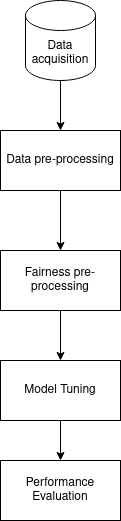
\includegraphics[width=.2\textwidth, height=0.6\textwidth]{FbD.png}
\end{center}
\newpage
In the following are presented the several algorithms that have been put into the \textbf{Fairness pre-processing} step to perform a final comparaison.
\section{Fairness through unawareness with proxy detection}
The algorithm presented in this section is rooted in the fundamental concept of "Fairness through Unawareness." This approach is underpinned by the overarching goal of mitigating bias by removing certain attributes from the dataset. Notably, in this scenario, the removal extends beyond solely the protected attributes, introducing a novel perspective on addressing bias. 

In the spirit of "Fairness through Unawareness," this approach advocates the removal of both the protected attributes and a set of proxy variables. These proxy variables serve as a distinctive feature of the algorithm, as they are strategically identified and eliminated alongside the protected attributes. The proxy variables are defined with a specific focus on aspects that could potentially introduce or perpetuate bias within the AI system. \cite{Gupta2018ProxyF}

The identification and removal of these proxy variables align with the commitment to promoting fairness and equity. By addressing not only the protected attributes but also the factors that may indirectly influence bias, this algorithm adopts a comprehensive approach to bias mitigation. 

The incorporation of proxy variables represents an innovative and proactive step within the workflow, enhancing the system's ability to address bias from multiple angles. This multifaceted approach contributes to the overarching mission of developing AI systems that are not only accurate but also equitable, just, and fair.

\subsection{Algorithm description}
In the following there is the description of the algorithm presented here in its two different versions: the one that comes out using the \textbf{apriori} algorithm and the one that comes out using \textbf{variables only} to perform proxy detection. 


Let's consider a dataset \( D \) belonging to \( \mathbb{R}^{n \times m} \) with \( k \) protected variables. 


\textit{fairness\_evaluation} is defined as follows:
\[
\text{fairness\_evaluation}(v_i, Y) = \lambda(v_i, Y) \quad \forall i \in [1, k]
\]

where:
\begin{align*}
v\_i & : \text{ith attribute belonging to the protected variables}, Y & : \text{output column}.
\end{align*}

The fairness function \( \lambda \) evaluates the relationship between a protected attribute \( v_i \) and the output \( Y \), producing a value that represents the level of fairness for that protected attribute. 


\textit{dataset\_fair} is defined as follows: a dataset \( D \) is considered fair if for every value \( v \) belonging to \textit{fairness\_evaluation}, the following condition holds:
\[ 0.8  < v < 1.25 \] 


Considering the relevance of proxy detection in this algorithm it's important to move on and define the two approaches to detect these variables. 


\subsubsection{Proxy detection via attributes only}
Let's consider the set \( A \), represented as the set of all variables in the dataset excluding the protected variables, and the set \( B \), representing the protected variables.

\textit{proxy\_detection} is defined as follows: for every variable \( \text{var} \) belonging to \( A \) and for every protected variable \( \text{var\_protected} \) belonging to \( B \), the variable is a proxy if the fairness metric \( \lambda(\text{var}, \text{var\_protected}) \) satisfies the condition:

\[
\lambda(\text{var}, \text{var\_protected}) <= 0.8 \quad \text{or} \quad \lambda(\text{var}, \text{var\_protected}) => 1.25
\]

In other words, a variable \( \text{var} \) is considered a proxy if the fairness measure \( \lambda \) between \( \text{var} \) and a protected variable \( \text{var\_protected} \) falls outside the acceptable range ]0.8, 1.25[. 


\subsubsection{Proxy detection via apriori}
It's important to give a brief background of the Association Rule Mining, the family algorithm \textbf{apriori} belongs to.

\begin{enumerate}
    \item \textbf{Association rule mining}:
    Association rule mining represents a pivotal data mining technique employed to unearth intriguing relationships and patterns hidden within extensive datasets. This technique is specifically tailored to the task of identifying associations and correlations among diverse elements present in the data, thereby revealing valuable insights and connections that might otherwise remain concealed. 

    The primary objective of association rule mining is to expose the inherent dependencies between data items or attributes. It scrutinizes the dataset in search of rules that reveal the co-occurrence and relationships between different items. These rules often manifest in the form of "if-then" statements, where the presence of one item is associated with the presence or absence of another. 

    This technique is particularly advantageous when applied to large volumes of data, as it excels in discovering subtle, non-obvious associations that might elude simple statistical analysis. Association rule mining is a versatile tool with a wide array of applications, spanning domains such as market basket analysis, recommendation systems, and fraud detection. 

    The process of association rule mining involves the generation of itemsets and the identification of frequent itemsets—combinations of items that appear together frequently. The algorithm then extracts association rules from these frequent itemsets, offering valuable insights into the relationships and co-occurrences within the data. 

    The outcomes of association rule mining have the potential to drive informed decision-making, such as product recommendations based on customer purchase history, optimizing supply chain management, and identifying suspicious patterns in financial transactions.
    

    \item \textbf{Apriori algorithm}: Suppose to have a set of transactions $T$, each containing a set of items. Let's define:

\begin{itemize}
  \item $I$: the set of all distinct items in the data.
  \item $D$: the set of transactions, each represented by a set of items.
  \item $F_k$: the set of frequent itemsets of length $k$.
\end{itemize}

The Apriori algorithm operates in iterations, generating $F_k$ from $F_{k-1}$.

\textbf{Step 1:} Initialization:
$$F_1 = \{ \text{frequent item } i, i \in I \}$$

\textbf{Step 2:} Candidate itemset generation:
$$C_k = \{ \text{set } c \text{ of items such that } c \subseteq F_{k-1} \}$$

\textbf{Step 3:} Database scan:
$$\text{For each transaction } t \text{ in } D, \text{ increment the support count of each candidate in } C_k \text{ contained in } t.$$

\textbf{Step 4:} Selection of frequent itemsets:
$$F_k = \{ c \in C_k \text{ such that the support of } c \geq \text{ specified threshold} \}$$

\item \textbf{Row Selection with a Confidence Level}: 
suppose to have obtained association rules using the Apriori algorithm. Each rule $R$ is in the form $A \rightarrow B$, where $A$ is the antecedent and $B$ is the consequent. The confidence of $R$ is defined as:

\[
\text{Confidence}(R) = \frac{\text{Support}(A \cup B)}{\text{Support}(A)}
\]

To select rows with a certain confidence level, is considered a confidence threshold $C_{\text{min}}$. If the confidence of a rule $R$ exceeds this threshold, the rule is accepted.

Formally, a rule $A \rightarrow B$ is accepted if:

\[
\text{Confidence}(A \rightarrow B) \geq C_{\text{min}}
\]
In our scenario
\[
C_{\text{min}}
\]
is equal to 0.8. 


The consequent filtering process involves evaluating each rule to ensure it meets this criteria. If the consequent of a rule does not contain any sensitive attributes, that rule is discarded from the final selection. 


Formally, a rule $A \rightarrow B$ is considered if:

\[
\exists b \in B : b \in S
\]

If this condition is not met, the rule is discarded from the final selection.
\end{enumerate}
After this brief introduction of the concepts used to apply this algorithm is presented the approach to detect proxy variables. 

\textit{proxy\_detection} is defined as follows: for each antecedent \( A_i \) belonging to the antecedent list \( \mathcal{A} \), for each consequent \( C_j \) belonging to the consequent list \( \mathcal{C} \), and for each protected variable \( V_k \) belonging to the protected variable list \( \mathcal{V} \), \( A_i \) is a proxy if the fairness metric \( \lambda(A_i, C_j) \) is such that:

\[\lambda(A_i, C_j) <= 0.8 \quad \text{or} \quad \lambda(A_i, C_j) >= 1.25\]

In other words, an antecedent \( A_i \) is considered a proxy if the fairness measure \( \lambda \) between \( A_i \) and a consequent \( C_j \) is outside the acceptable range ]0.8, 1.25[.




There are two other fucnctions that needs to be defined in order to complete our algorithm.




Considering the dataset \( D \) belonging to \( \mathbb{R}^{n \times m} \) and \( k \) as the number of identified proxy variables, the function \( \text{proxy\_free\_dataset} \) is defined as follows:

\[
\text{\textbf{proxy\_free\_dataset}}: D \times \mathbb{R}^{k \times 1} \rightarrow \mathbb{R}^{n \times (m - k)}
\]

where \( j = m - k \) and \( \text{proxy\_free\_dataset}(D) \) yields a dataset \( \mathbb{R}^{n \times j} \) devoid of the proxy variables, ensuring the removal of any potential indirect indicators that may influence sensitive attributes. 



Considering the dataset \( D \) belonging to \( \mathbb{R}^{n \times j} \) where j are the columns obtained after the proxy removals and \( k \) as the number of identified protected variables, the function \( \text{protected\_attributes\_free\_dataset} \) is defined as follows:

\[
\text{\textbf{protected\_attributes\_free\_dataset}}: D \times \mathbb{R}^{k \times 1} \rightarrow \mathbb{R}^{n \times (j - k)}
\]

where \( p = j - k \) and \( \text{protected\_attributes\_free\_dataset}(D) \) yields a dataset \( \mathbb{R}^{n \times p} \) devoid of the protected variables, ensuring the removal of any potential indirect indicators that may influence sensitive attributes.

\subsection{Pseudocode}
Here's the pseudocode of the \emph{Fairness through unawareness with proxy detection}:

\begin{algorithm}[H]
    \KwData{dataset}
    \KwResult{fair dataset}
    \While{\textbf{not} \textit{dataset\_fair(dataset)} \textbf{or} \textit{protected\_attributes} \textbf{in} \textit{dataset}}{
        proxies = \textit{proxy\_detection(dataset)}\;
        \If{proxies \textbf{is empty}}{
            dataset = \textit{protected\_attributes\_free\_dataset(dataset)}\;
        }
        \Else{
            dataset = \textit{proxy\_free\_dataset(dataset)}\;
        }
    }
    \KwRet{dataset}
\end{algorithm}

\subsubsection{dataset\textunderscore fair pseudocode}
Here's the pseudocode that establish if the dataset is either \emph{Fair} or not

\begin{algorithm}[H]
    \KwData{dataset, protected\_attribute}
    \KwResult{Boolean value indicating fairness}
    \If{\textit{fairness\_evaluation(dataset, protected\_attribute)} \textbf{is empty}}{
        \KwRet{\textbf{True}}\;
    }
    \KwRet{\textbf{False}}
\end{algorithm}

\subsubsection{fairness\textunderscore evaluation pseudocode}
Here's the pseudocode to perform the fairness evaluation, given a specific \emph{fairness metric}

\begin{algorithm}[H]
    \KwData{dataset, output\_column, protected\_attributes}
    \KwResult{List of attributes failing fairness evaluation}
    fairness\_evaluation\_list $\gets$ empty list\;
    output $\gets$ dataset[output\_column]\;
    \For{attribute \textbf{in} protected\_attributes}{
        \If{\textit{metric(attribute, output)} $\leq$ 0.8 \textbf{or} \textit{metric(attribute, output)} $\geq$ 1.25}{
            \textit{fairness\_evaluation\_list.append(attribute)}\;
        }
    }
    \KwRet{fairness\_evaluation\_list}
\end{algorithm}

\subsubsection{protected\textunderscore attributes\textunderscore free\textunderscore dataset pseudocode}
Here's the pseudocode to remove protected attributes from the dataset

\begin{algorithm}[H]
    \KwData{dataset, protected\_attributes}
    \KwResult{Dataset with protected attributes removed}
    \For{attribute \textbf{in} protected\_attributes}{
        \textit{dataset.remove(attribute)}\;
    }
    \KwRet{dataset}
\end{algorithm}

\subsubsection{proxy\textunderscore free\textunderscore dataset pdeudocode}
Here's the pseudocode to remove proxy attributes from the dataset

\begin{algorithm}[H]
    \KwData{dataset, proxy\_list}
    \KwResult{Dataset with proxies removed}
    \For{proxy \textbf{in} proxy\_list}{
        \textit{dataset.remove(proxy)}\;
    }
    \KwRet{dataset}
\end{algorithm}

\subsubsection{proxy\textunderscore detection pseudocode}
Here's the pseudocode of proxy\textunderscore detection function. There are 2 scenarios that are presented here, the one in which the \emph{variables only}  approach is used and the one in which the \emph{apriori} approach is used

\begin{enumerate}
    \item \textbf{Variables only}: 
            
\begin{algorithm}[H]
    \KwData{protected\_attributes\_list, attributes}
    \KwResult{List of proxies}
    proxy\_list $\gets$ empty list\;
    \For{protected\_attribute \textbf{in} protected\_attributes\_list}{
        \For{attribute \textbf{in} attributes \textbf{and not in} protected\_attributes\_list \textbf{and not in} proxy\_list}{
            \If{\textit{metric(attribute, protected\_attribute)} $\leq$ 0.8 \textbf{or} \textit{metric(attribute, protected\_attribute)} $\geq$ 1.25}{
                \textit{proxy\_list.append(attribute)}\;
            }
        }
    }
    \KwRet{proxy\_list}
\end{algorithm}

    \item \textbf{Apriori}:

    \begin{algorithm}[H]
    \KwData{apriori\_dataset}
    \KwResult{List of proxies}
    proxy\_list $\gets$ empty list\;
    \For{consequent \textbf{in} apriori\_dataset}{
        \For{antecedent \textbf{in} apriori\_dataset}{
            \If{\textit{metric(antecedent, consequent)} $\leq$ 0.8 \textbf{or} \textit{metric(antecedent, consequent)} $\geq$ 1.25}{
                \textit{proxy\_list.append(antecedent)}\;
            }
        }
    }
    \KwRet{proxy\_list}
\end{algorithm}
\end{enumerate}
\newpage

\section{Fairness through data rebalancing}

In this approach, the paradigm of bias mitigation takes on a unique and innovative perspective, one that prioritizes data augmentation over attribute removal. Unlike traditional approaches that center on the exclusion of specific attributes, this methodology embraces the concept of data augmentation, introducing a distinctive definition of fairness and equity within the AI system.

The essence of this approach revolves around the augmentation of the dataset by introducing new data instances that offer a more comprehensive and inclusive representation of the underlying population. This expanded dataset is designed to be more diverse, representative, and balanced, transcending the limitations of the original data and fostering a more nuanced understanding of fairness. 

The introduction of augmented data instances leads to a redefined notion of fairness within the AI system. Instead of solely focusing on the absence of biased attributes, fairness is now measured in terms of the dataset's inclusivity and its ability to capture the diversity and nuances present within the population it seeks to serve. 

This approach aligns with the broader philosophy of ensuring that AI systems are equitable, just, and capable of making informed and unbiased decisions. By augmenting the dataset, it strives to bridge the gaps in representation and provide a more equitable playing field for all individuals, regardless of their background or characteristics. 

The process of data augmentation necessitates a careful selection of techniques and methodologies that can introduce new data instances while maintaining the integrity and quality of the dataset. These techniques may encompass oversampling, synthetic data generation, or other data synthesis methods, each tailored to the specific context and objectives of the AI system.

\subsection{A New Definition of Fairness}

In traditional fairness definitions, the focus often revolves around ensuring fair treatment for individual protected attributes, denoted as $A_1, A_2, \ldots, A_k$. While this is undoubtedly crucial, a more comprehensive understanding of fairness calls for an examination of fairness in the context of combinations of protected attributes and the output. A new definition of fairness is proposed, which takes into account the representation of all combinations of $k$ protected attributes and the output, aiming for equitable representation across these combinations.

\subsubsection{Equal Representation of Combinations}

A fair dataset is defined as one in which, for each combination of protected attributes $\{A_1, A_2, \ldots, A_k\}$ and the output $O_j$, the representation is equal and proportional. Mathematically, a dataset is fair if:

\[
\forall i_1, i_2, \ldots, i_k, j: \frac{|D_{i_1, i_2, \ldots, i_k, j}|}{|D|} = \text{constant}
\]

where:
- $D$ is the dataset,
- $|D_{i_1, i_2, \ldots, i_k, j}|$ is the number of samples with the specific combination of protected attributes $A_{i_1}, A_{i_2}, \ldots, A_{i_k}$ and output $O_j$,
- $|D|$ is the total number of samples in the dataset.

This entails that any combination of demographic groups, defined by the protected attributes, and the output should have comparable representation, thereby fostering a balanced and unbiased dataset.

\subsubsection{Promoting Comprehensive Fairness}

By striving for equal representation of combinations of protected attributes, is addressed a fundamental aspect of fairness that transcends individual attributes. This approach provides a more nuanced understanding of fairness by considering the intersections of various demographic groups. It encourages a broader examination of potential biases that may arise when considering multiple attributes simultaneously.

Incorporating this definition of fairness into the dataset rebalancing process enables us to promote a comprehensive notion of fairness, aligning with the principles of equal opportunity and non-discrimination across all combinations of protected attributes. Our subsequent algorithm and experimental evaluation are designed to actualize this definition and demonstrate its effectiveness in achieving a more equitable representation within the dataset.

\subsection{Algorithm description}

Let \( D \) be a dataset \( R^{n \times m} \), where \( n \) is the number of samples and \( m \) is the number of features. Let \( k \) be the number of protected variables represented as \( R^{n \times 1} \), and let there be a single output variable represented as \( R^{n \times 1} \).

A rebalancing function \( \mathcal{R} \) can be formally defined as a mapping:

\[
\mathcal{R}: R^{n \times m} \rightarrow R^{l \times m}
\]

where \( l > m \), and the function \( \mathcal{R} \) transforms the input dataset \( D \) of dimensions \( n \times m \) into an output dataset \( D' \) of dimensions \( l \times m \).



Let \( k \) be the number of binary protected variables in the dataset \( D \), and consider the output variable to be binary as well. The number of possible combinations of these variables is \( 2^{(k+1)} \).

Consider a set \( \text{Combination-frequency} \) with occurrences of all \( 2^{(k+1)} \) combinations within the dataset. For each combination, the number of rows in which that combination appears should be equal to the maximum occurrence among all combinations present in the set \( \text{Combination\textunderscore frequency} \). This maximum value is denoted as \( \text{Max}(\text{Combination-frequency}) \).

Mathematically, the number of rows (\( l \)) the final dataset should have for each combination is given by:

\[
l = \text{Max}(\text{Combination-frequency})
\]



Let \( l \) be the desired number of rows for the final dataset. For each combination of values, is calculated the occurrence count \( \text{occurrence}_i \), where \( i \) ranges from 1 to \( 2^{(k+1)} \), with \( k \) being the number of protected binary variables and considering the output variable as binary.

The total number of rows to be added is given by:

\[
\text{total\_rows\_to\_add} = l - \sum_{i=1}^{2^{(k+1)}} \text{occurrence}_i
\]

For each iteration:
\begin{itemize}
    \item The values of the protected and output variables are set according to the specific combination.
    \item For all other attributes, a random value \( \text{random\_value}_{ij} \) is generated, where \( j \) represents the specific attribute and \( i \) represents the row being added for that attribute. \( \text{random\_value}_{ij} \) is within the minimum and maximum range for attribute \( j \).
\end{itemize}

\subsection{Pseudocode}
\begin{algorithm}[H]
    \SetKwInOut{Input}{Input}
    \SetKwInOut{Output}{Output}

    \Input{combination\_set, combination\_frequency, protected\_attributes, dataset\_attributes}
    \Output{Updated dataset}

    max\_frequency $\gets$ max(combination\_frequency)\;
    \For{index $\gets$ 0 \KwTo len(combination\_set)}{
        combination $\gets$ combination\_set[index]\;
        frequency $\gets$ combination\_frequency[index]\;
        \While{frequency $<$ max\_frequency}{
            new\_row $\gets$ empty\;
            \For{(attr, val) \textbf{in} (combination, protected\_attributes)}{
                new\_row[attr] $\gets$ val\;
            }
            \For{attr \textbf{in} dataset\_attributes \textbf{and not in} protected\_attributes}{
                new\_row[attr] $\gets$ random(min(attr), max(attr))\;
            }
            dataset.add(new\_row)\;
            frequency $+$= 1\;
        }
    }
\end{algorithm}
\newpage
%----------------------------------------------------------------------------------------
%\chapter{Implementation} % possible chapter for Projects
%\label{chap:implementation}
%----------------------------------------------------------------------------------------
\section{Dataset description}
Before delving into the intricate details of the algorithm implementations presented earlier, it is imperative to provide a comprehensive overview of the dataset on which these algorithms have been applied. The chosen dataset for this work is the "ULL dataset," an invaluable resource that underpins the empirical exploration of bias mitigation strategies in the context of the educational system in the Canary Islands. 

The ULL dataset is a rich and expansive repository of information, meticulously compiled to capture various facets of the educational landscape within the Canary Islands. This dataset comprises the comprehensive census of students enrolled over four distinct academic years, offering a multifaceted glimpse into the educational ecosystem. 

The dataset encompasses a diverse array of attributes and data points, encapsulating critical information such as student demographics, academic performance, socioeconomic factors, and other pertinent variables. These attributes collectively provide a holistic perspective on the educational landscape, enabling a nuanced analysis of the factors that influence student outcomes and experiences. 

The temporal dimension of the dataset, spanning four academic years, further enriches the analytical potential. It allows for the investigation of temporal trends, shifts in educational policies, and the evolution of student characteristics over time. This temporal depth is particularly valuable when examining the efficacy of bias mitigation strategies, as it facilitates the assessment of their impact across different academic years. 

The ULL dataset is not merely a repository of numbers and statistics; it is a window into the educational opportunities and challenges faced by students in the Canary Islands. By harnessing the insights gleaned from this dataset, it becomes possible to proactively address biases and promote equity within the educational system, ultimately striving for a more inclusive and just educational landscape.

\subsection{Pre-processing operations on ULL dataset}
A deep analysis of the dataset led us to make a first features selection. More specifically for this work only the \emph{important} and \emph{protected} attributes have been selected.
\subsubsection{Protected attributes choice}
After a proper domain analysis the protected attributes selected to be passed to the algorithms have been a subset of the orginal selected:
\begin{enumerate}
    \item sex
    \item capital island: if the student comes from the capital of the city
    \item public\textunderscore private: if the school is public or private
    \item inmigrant: if the student is either inmigrant or not
    \item inmigrant second gen: if the student is either inmigrand of second gen or not
    \item parent expectation
    \item mothly houseold income
    \item cconomic, social and cultural satus index
\end{enumerate}
\subsubsection{Attributes pre-processing}
The dataset documentation provided the information related to the type of each attribute (e.g. Continuous or Categorical). Starting from this information the variables have been pre-processed as follows.
\begin{itemize}
    \item Each categorical attribute has been replaced with an encoded value
    \item For each protected attribute has been computed the following operation:
    \begin{itemize}
        \item If the protected attirbute is a binary one, assuming that the binary values may not be onlu 0 and 1, then the greatest value has been replaced with 1 and the other one with 0.
        \item If the protected attribute is a categorical one then is performed a search of the most frequent value in the column. Then this value in the column is replaced with 1, otherwise with 0. With this policy is established that the fairness must be guaranteed between the most frequent value and the others.
        \item if the protected attribute is a continuous one then is computed the the theshold resulting from the sum of minimum value and maximum value in the column divided by 2. Every value in the column above this threshold is replaced with 1, otherwise with 0. This means that the fairness must be guaranteed between the students that are above the threshold for a specific attribute and the other ones.
    \end{itemize}
\end{itemize}

\subsection{Goal of this work}
The several output in this dataset are considered as protected attributes. More specifically the goal of this work is to predict the english level of a given student. Since the \emph{level\textunderscore ing} attribute is a categorical ones then the output states if a student has the same level of the majority of the students or if not. The goal is to make the predictor and the prediction fair, this means that the belonging of a student to a specific output, the match indeed, must no be influenced by any other factors rather than the predictor's mechanisms.
\newpage
\section{Fairness through unawareness with proxy detection: implementation}
In this section are reported the several implementative issues and features that have been encountered and designed during the development of this algorithm. Two approaches are explored in detail, the one with \textbf{apriori} and the one in which only the \textbf{variables} have been taken in account. 

Before moving on it's important to be more detailed about the fairness metric used, expecially in the \emph{Fairness through unawareness with proxy detection} algorithm 
\subsection{Disparate Impact}
Disparate Impact (DI) is a pivotal fairness metric widely employed in the context of algorithmic decision-making and predictive modeling. It is meticulously designed to assess and quantify the potential discriminatory effects of a decision-making process on different demographic groups, providing a quantitative means of gauging fairness and equity. 

The essence of DI revolves around the principle that a fair decision-making process should not disproportionately disadvantage any specific demographic group. In other words, it evaluates whether a model's predictions or decisions adversely affect certain groups more than others. To calculate DI, one typically examines the outcomes generated by an AI system for distinct demographic subgroups and compares the proportions of favorable outcomes. 

The DI metric is mathematically expressed as the ratio of the proportion of favorable outcomes for the disadvantaged group to the proportion of favorable outcomes for the advantaged group. If this ratio is close to 1, it indicates that the model's decisions are roughly equally favorable across demographic groups, implying a fair process. However, if the ratio significantly deviates from 1, it suggests that there may be disparities in the impact of the AI system on different groups, signifying potential bias or discrimination.

The mathematical definition is:
\[
\text{Disparate Impact (DI)} = \frac{P(\text{Favorable Outcome} | \text{Disadvantaged Group})}{P(\text{Favorable Outcome} | \text{Advantaged Group})}
\]

where $P(\text{Favorable Outcome} | \text{Disadvantaged Group})$ is the probability of a favorable outcome given membership in the disadvantaged group, and  
 $P(\text{Favorable Outcome} | \text{Advantaged Group})$ is the probability of a favorable outcome given membership in the advantaged group.
\subsection{Proxy detection via apriori}
The implementation of this approach has proceeded according a modular approach and, more specifically, has been developed a module named \emph{fairness} in which there are all the sub-modules needed to implement this approach.
\subsubsection{fairness\textunderscore metric module}
This module has been thought to contain the implementation of the several fairness metrics considered in the context of the study. In our scenario it only contains the implementation of the \emph{Disparate Impact} metric. 

This implementation provides to the user the information about the fairness status of the dataset provided together with the protected attributes, the otuput attribute and the possible values that this value may have: 

\begin{lstlisting}
    def fairness_evaluation(self, dataset: pd.DataFrame, protected_attributes: list, output_column_values: list,
                            output_column: str) -> str:
        """
        This method perform an evaluation of the fairness of a given dataset according to the Disparate Impact metric
        :param dataset: this is the dataset on which to be labelled as fair or unfair
        :param protected_attributes: the list of the protected attributes on which compute the disparate impact value
        :param output_column: the column of the dataset that represents the output
        :return: return 'fair' if the dataset is fair, unfair 'otherwise'
        """
        bias_analysis_dataframe = self.bias_detection(dataset, protected_attributes, output_column_values, output_column)
        return_value = 'unfair'
        for value in bias_analysis_dataframe['Disparate Impact'].values:
            if value <= 0.80 or value >= 1.25:
                return_value = 'unfair'
                break
            else:
                return_value = 'fair'

        return return_value
\end{lstlisting}


\subsubsection{matching module}
This module only contains the method \emph{conscious\textunderscore fairness\textunderscore through\textunderscore unawareness} that can return the dataset in two possible configurations:
\begin{enumerate}
    \item if the dataset is fair it returns the dataset itself only with variables pre-processed. Since these pre-processing operations are performed before the fairness checking these are the same for both scenarios. These operations are the transformation of every \emph{categorical} attribute into a numerical one and the transformation of protected attributes as explained above.
    \item if the dataset is not fair the algorithm looks for the proxies and remove the proxies found if there are some and the protected attributes.
\end{enumerate}
\subsubsection{proxy module}
This module is the core of the whole algorithm. This module contains other two sub-modules. More specifically it contains a module whose goal is to detect proxy and the other one is the module in charge to translate the result of the proxy detection to provide a list of proxies to be used into the \emph{matching} module
\begin{enumerate}
    \item \emph{proxy\textunderscore detection}: this module is the one in which the \emph{apriori} algorithm is applied in order to found the relation between antecedents and consequents with a confidence value of 0.8. The key method of this module is the private method \emph{\textunderscore return\textunderscore apriori\textunderscore dataframe}. This method performs computation on the result of the application of the apriori algorithm. More specifically it returns a dataframe with 3 columns \textbf{Antecedent}, \textbf{Consequent}, \textbf{Confidence} 

    \begin{lstlisting}
        def _return_apriori_dataframe(association_results: list) -> pd.DataFrame:
    """This function returns the dataframe with the association generated by the apriori algorithm

    Args:
        association_results (list): is the list of the association returned by the apriori algorithm

    Returns:
        pd.DataFrame: is the dataframe equivalent to the association result list
    """
    antecedent = []
    consequent = []
    confidence = []

    for association_result in association_results:
        for ordered_statistic in association_result.ordered_statistics:
            antecedent_elements = list(ordered_statistic.items_base)
            antecedent.append(antecedent_elements)
            consequent_elements = list(ordered_statistic.items_add)
            consequent.append(consequent_elements)
            confidence_elements = ordered_statistic.confidence
            confidence.append(confidence_elements)

    antecedent_series = pd.Series(antecedent)
    consequent_series = pd.Series(consequent)
    confidence_series = pd.Series(confidence)

    dataframe = pd.DataFrame(
        {'Antecedent': antecedent_series, 'Consequent': consequent_series, 'Confidence': confidence_series})

    return dataframe
    \end{lstlisting}
    \item \emph{proxy\textunderscore processing}: this module contains two key methods. The first method, \emph{\textunderscore return\textunderscore proxy\textunderscore protected\textunderscore attribute} returns a dataframe in which for each sensitive attribute as consequent are related the antecedents that are the possible proxies for that sensitive attribute. The second method is \emph{proxy\textunderscore fixing}, in which for each antecedent is computed the Disparate impact value related to that consequent with that specific value. Only the variables with DI value lesser than 0.8 or greater than 1.25 are considered as proxies. In the following is reported the code of both methods:
    \begin{lstlisting}
        def _return_proxy_protected_attribute(proxy_variables: pd.DataFrame, protected_attributes: list) -> pd.DataFrame:
    """This method returns a dataframe containing the proxy variables for each sensitive attribute

    Args:
        proxy_variables (pd.DataFrame): the dataframe of the proxy variables (antecedent, consequent, confidence)
        protected_attributes (list): the list of the protected attributes

    Returns:
        pd.DataFrame: _description_
    """
    sensitive_antecedent = []
    sensitive_consequent = []
    for index, proxy_row in proxy_variables.iterrows():
        for consequent in proxy_row['Consequent']:
            for sensitive_attribute in protected_attributes:
                if str(consequent).startswith(sensitive_attribute):
                    sensitive_antecedent.append(proxy_row['Antecedent'])
                    sensitive_consequent.append(consequent)

    dataframe = pd.DataFrame(
        {'Antecedent': pd.Series(sensitive_antecedent), 'Consequent': pd.Series(sensitive_consequent)})

    return dataframe


    \end{lstlisting}
    \begin{lstlisting}
        def proxy_fixing(original_dataset: pd.DataFrame, 
        protected_attributes: list) -> pd.DataFrame:
    """This method returns a dataset with proxy variables founded in the original dataset analyzed.
    In case these proxies lead to unfairness the proxies are deleted

    Args: original_dataset (pd.DataFrame): the dataset on which the proxy variable have to be deleted if they lead to
    unfairness
    protected_attributes (list): the list of protected attribute on which perform the proxy analysis

    Returns:
        pd.DataFrame: returns the dataframe in which the proxies do not lead to fairness
    """
    proxy_variables = return_proxy_variables(original_dataset)
    proxy_variables_for_sensitive_attributes = 
    _return_proxy_protected_attribute(proxy_variables, protected_attributes)
    
    dataset = original_dataset
    for index, row in proxy_variables_for_sensitive_attributes.iterrows():
        for antecedent in row['Antecedent']:
            consequent = row['Consequent']

            disparate_impact_value = _compute_disparate_impact_for_proxy(
                antecedent, consequent,original_dataset)

            if not 0.8 < disparate_impact_value < 1.25 and _proxy_format_to_column(antecedent) not in protected_attributes:
                dataset = _remove_proxy_from_dataset(original_dataset, antecedent)

            else:
                continue

    return dataset

    \end{lstlisting}
\end{enumerate}

\subsection{Proxy detection via variables only: implementation}
The implementation of this approach differs with the implementation of the apriori approach because of the operation of proxy detection and processing have been mixed together and the proxy removal operation has been delegated to the \emph{matching} module. In the following there's the code that computes the proxy detection:
\begin{lstlisting}
    def proxy_detection(dataset: pd.DataFrame, protected_attributes: list, output_column: str) -> list:
    attributes_list = []
    for attr in dataset.columns:
        if attr not in protected_attributes:
            attributes_list.append(attr)
            
          
    if output_column in attributes_list:
        attributes_list.remove(output_column)
        
    proxy_list = []
    for attribute in attributes_list:
        for protected_attribute in protected_attributes:
            if _compute_disparate_impact_for_proxy(attribute, protected_attribute, dataset) == 'PROXY':
                proxy_list.append(attribute)

    return proxy_list

\end{lstlisting}
\newpage
\section{Fairness through data rebalancing: implementation}
The first big difference between this approach and the two previous ones is that no fairness-metrics is used here. The reason behind this is the new definition provided for fairness, where is assumed as a parity in combination occurrance. So the core of this algorithm is the \emph{rebalancing} module in which rows are added to the dataset according to the most frequent combination occurrance in the original dataset.
The key part of this module is the one in which the other attributes are inserted. In this scenario a new value is added considering the minimum and the maximum in the temporary dataset, where this dataset is the dataset in which a certain combination of protected\textunderscore attributes and output is occurred. It's furthermore important to remark that since a value has been  randomically chosen this may alter the distribution for that attribute.
\begin{lstlisting}
    for index in range(0, len(combination_list)):
        combination = combination_list[index]
        temp_dataset = final_dataset.query(return_query_for_dataframe(combination, combination_attributes))
        if combination_frequency[index] == combination_frequency_target:
            continue
        else:
            for counter in range(0, combination_frequency_target - combination_frequency[index]):
                new_row = {}
                for (attr, value) in zip(combination_attributes, combination):
                    new_row[attr] = value
                for attribute in final_dataset.columns:
                    if attribute not in combination_attributes:
                        if is_variable_discrete(temp_dataset, attribute):
                            new_row[attribute] = random.randint(temp_dataset[attribute].min(), temp_dataset[attribute].max())
                        else:
                            new_row[attribute] = random.uniform(temp_dataset[attribute].min(), temp_dataset[attribute].max())
                
                final_dataset.loc[len(final_dataset)] = new_row

\end{lstlisting}

%----------------------------------------------------------------------------------------
\chapter{Validation} % possible chapter for Projects
\label{chap:validation}
%----------------------------------------------------------------------------------------
Following the information reported into the \emph{Dataset} section the models presented in the following have been trained with the goal to predict wether the english level is above or behind the thershold. 

For each grade have been applied the following approaches, in order to perform a proper comparaison:
\begin{enumerate}
    \item No fairness assumptions are made
    \item Fairness through unawareness
    \item Fairness through unawareness with proxy detection via apriori
    \item Fairness through unawareness with proxy detection via variables only
    \item Fairness through data rebalancing
\end{enumerate}

\section{Experiment setup}
For each of the previous approaches have been chosen 3 models to perform the prediction:
\begin{enumerate}
    \item \text{RandomForest Classifier}: RandomForest Classifier is a popular machine learning algorithm that leverages an ensemble of decision trees to make predictions. It excels at tasks like classification and regression, offering robustness against overfitting and high accuracy by aggregating the predictions of multiple decision trees. It's a versatile tool used in various applications, from finance to healthcare and image analysis.
    \item \textbf{XGBoost Classifier}: XGBoost, short for "Extreme Gradient Boosting," is a powerful and efficient machine learning algorithm known for its exceptional predictive performance. It's a gradient boosting technique that builds a strong predictive model by combining the predictions of multiple weak models, typically decision trees. XGBoost is widely used in data science and machine learning competitions due to its speed, accuracy, and flexibility. It can handle both regression and classification tasks and is prized for its ability to handle large datasets and complex relationships in the data.
    \item \textbf{DecisionTree Classifier}: DecisionTree Classifier is a specific type of machine learning algorithm primarily used for classification tasks. It constructs a tree-like model, where each internal node represents a decision based on a specific feature, and each leaf node denotes the predicted class label for the input data point.
\end{enumerate}

On the previous models is applied the GridSearch with a \emph{cv} of 10 in order to select the best parameters combination for each one. In the following are reported the specific parameters for each model:
\begin{enumerate}
    \item RandomForest Classifier:
    \begin{enumerate}
        \item \emph{n\textunderscore estimators}: [10, 100, 10]
        \item \emph{criterion}: [gini, entropy, log\textunderscore loss]
        \item \emph{max\textunderscore depth}: [10, 50, 10]
        \item \emph{max\textunderscore leaf\textunderscore nodes}: [10, 50, 10]
    \end{enumerate}
    \item XGBoost Classifier:
    \begin{enumerate}
        \item \emph{min\textunderscore child\textunderscore weight}: [1, 5, 10]
        \item \emph{gamma}: [0.5, 1, 1.5, 2.5]
        \item \emph{subsample}: [0.6, 0.8, 1.0]
        \item \emph{colsample\textunderscore bytree}: [0.6, 0.6, 1.0]
        \item \emph{max\textunderscore depth}: [3, 4, 5]
    \end{enumerate}
    \item DecisionTree Classifier:
    \begin{enumerate}
        \item \emph{criterion}: [gini, entropy, log\textunderscore loss]
        \item \emph{max\textunderscore depth}: [10, 50, 10]
        \item \emph{max\textunderscore leaf\textunderscore nodes}: [10, 50, 10]
    \end{enumerate}
\end{enumerate}

Each model is trained with the 67\% of the dataset while the 33\% is left for the test.
In the following are reported the results for each grade. More specifically for each model is reported the best model selected and the accuracy on the test set.
\newpage
\section{Grade 3}
\subsection{No-fair approach}
\subsubsection{Best models}
\begin{tabular}{|c|c|}
    \hline
    \textbf{Model} & \textbf{Best parameters} \\
    \hline
    RandomForest Classifier  &  \\
    \hline
    XGBoost Classifier & \\
    \hline
    DecisionTree Classifier & \\
    \hline
\end{tabular}

\subsubsection{Accuracy}
\begin{tabular}{|c|c|}
    \hline
    \textbf{Model} & \textbf{Accuracy} \\ 
    \hline
    RandomForest Classifier  &  \\
    \hline
    XGBoost Classifier & \\
    \hline
    DecisionTree Classifier & \\ 
    \hline
\end{tabular}

\subsection{Fairness throguh unawareness}
\subsubsection{Best models}
\begin{tabular}{|c|c|}
    \hline
    \textbf{Model} & \textbf{Best parameters} \\
    \hline
    RandomForest Classifier  &  \\
    \hline
    XGBoost Classifier & \\
    \hline
    DecisionTree Classifier & \\ 
    \hline
\end{tabular}

\subsubsection{Accuracy}
\begin{tabular}{|c|c|}
    \hline
    \textbf{Model} & \textbf{Accuracy} \\
    \hline
    RandomForest Classifier  &  \\
    \hline
    XGBoost Classifier & \\
    \hline
    DecisionTree Classifier & \\ 

    \hline
\end{tabular}

\subsection{Fairness through unawareness with proxy detection via apriori}
\subsubsection{Best models}
\begin{tabular}{|c|c|}
    \hline
    \textbf{Model} & \textbf{Best parameters} \\
    \hline
    RandomForest Classifier  &  \\
    \hline
    XGBoost Classifier & \\
    \hline
    DecisionTree Classifier &  \\
    \hline
\end{tabular}

\subsubsection{Accuracy} 
\begin{tabular}{|c|c|}
    \hline
    \textbf{Model} & \textbf{Accuracy} \\ 
    \hline
    RandomForest Classifier  &  \\
    \hline
    XGBoost Classifier & \\
    \hline
    DecisionTree Classifier & \\ 
    \hline
\end{tabular}

\subsection{Fariness through unawareness with proxy detection via variables only}
\subsubsection{Best models}
\begin{tabular}{|c|c|}
    \hline
    \textbf{Model} & \textbf{Best parameters} \\
    \hline
    RandomForest Classifier  &  \\
    \hline
    XGBoost Classifier & \\
    \hline
    DecisionTree Classifier & \\ 
    \hline
\end{tabular}

\subsubsection{Accuracy}
\begin{tabular}{|c|c|}
    \hline
    \textbf{Model} & \textbf{Accuracy} \\ 
    \hline
    RandomForest Classifier  &  \\
    \hline
    XGBoost Classifier & \\
    \hline
    DecisionTree Classifier & \\ 
    \hline
\end{tabular}

\subsection{Fairness through data rebalancing}
\subsubsection{Best models}
\begin{tabular}{|c|c|}
    \hline
    \textbf{Model} & \textbf{Best parameters} \\
    \hline
    RandomForest Classifier  &  \\
    \hline
    XGBoost Classifier & \\
    \hline
    DecisionTree Classifier & \\ 
    \hline
\end{tabular}

\subsubsection{Accuracy}
\begin{tabular}{|c|c|}
    \hline
    \textbf{Model} & \textbf{Accuracy} \\
    \hline
    RandomForest Classifier  &  \\
    \hline
    XGBoost Classifier & \\
    \hline
    DecisionTree Classifier & \\ 
    \hline
\end{tabular}

\iffalse
\newpage
\section{Grade 4}
\subsection{Best models}
\begin{tabular}{|c|c|}
    \hline
    \textbf{Model} & \textbf{Best parameters} 

    \hline
    RandomForest Classifier  &  

    \hline
    XGBoost Classifier & 

    \hline
    DecisionTree Classifier &  

    \hline
\end{tabular}

\subsection{Accuracy}
\begin{tabular}{|c|c|}
    \hline
    \textbf{Model} & \textbf{Accuracy} 

    \hline
    RandomForest Classifier  &  

    \hline
    XGBoost Classifier & 

    \hline
    DecisionTree Classifier &  

    \hline
\end{tabular}

\newpage
\section{Grade 6}
\subsection{Best models}
\begin{tabular}{|c|c|}
    \hline
    \textbf{Model} & \textbf{Best parameters} 

    \hline
    RandomForest Classifier  &  

    \hline
    XGBoost Classifier & 

    \hline
    DecisionTree Classifier &  

    \hline
\end{tabular}

\subsection{Accuracy}
\begin{tabular}{|c|c|}
    \hline
    \textbf{Model} & \textbf{Accuracy} 

    \hline
    RandomForest Classifier  &  

    \hline
    XGBoost Classifier & 

    \hline
    DecisionTree Classifier &  

    \hline
\end{tabular}
\fi

%----------------------------------------------------------------------------------------
\chapter{Conclusion}
\label{chap:conclusions}
%----------------------------------------------------------------------------------------

Write conclusions here.


%----------------------------------------------------------------------------------------
% BIBLIOGRAPHY
%----------------------------------------------------------------------------------------

\backmatter

%\nocite{*} % comment this to only show the referenced entries from the .bib file

\bibliographystyle{alpha}
\bibliography{bibliography}


\end{document}